\documentclass[acmtog, 11pt]{acmart}

%% Remove Citation Info
\settopmatter{printacmref=false} % Removes citation information below abstract
\renewcommand\footnotetextcopyrightpermission[1]{} % removes footnote with conference information in first column
\pagestyle{plain} % removes running headers
\makeatletter
\renewcommand\@formatdoi[1]{\ignorespaces}
\makeatother
%%


\usepackage{booktabs} % For formal tables

% TOG prefers author-name bib system with square brackets
\citestyle{acmnumeric}
\setcitestyle{square}


\usepackage[ruled]{algorithm2e} % For algorithms
\renewcommand{\algorithmcfname}{ALGORITHM}
\SetAlFnt{\small}
\SetAlCapFnt{\small}
\SetAlCapNameFnt{\small}
\SetAlCapHSkip{0pt}
\IncMargin{-\parindent}

% Metadata Information
\acmYear{2018}
\acmMonth{4}

% Copyright
%\setcopyright{acmcopyright}
%\setcopyright{acmlicensed}
%\setcopyright{rightsretained}
%\setcopyright{usgov}
\setcopyright{usgovmixed}
%\setcopyright{cagov}
%\setcopyright{cagovmixed}

% DOI
\acmDOI{}
% Set figure folder path
\graphicspath{{./figures/}}

% Document starts
\begin{document}
% Title portion
\title{Content-Based LSTM Network for Estimating Music Play Counts}

\author{Kyle Salitrik}
\affiliation{%
  \institution{The Pennsylvania State University}
  \city{State College}
  \state{PA}
  \postcode{16801}
  \country{USA}}
\author{Tomoki Takasawa}
\affiliation{%
  \institution{The Pennsylvania State University}
  \city{State College}
  \state{PA}
  \postcode{16801}
  \country{USA}}


\begin{abstract}
In the current state of the music industry, about 1\% of artists make up nearly 80\% of the total revenue in the market. The aim of our research is to create an assistant for recommendation systems that estimates the number of times a song would be played by a particular user, and therefore generate the most revenue for artists. By utilizing only audio data, we construct a system that is ignorant of an artist's popularity or other metadata such as genre. It provides a win-win-win situation for musicians, consumers, and record labels: Users will be able to discover new artists, up-and-coming artists could be recommended more often and allow them to gain a larger fanbase, and record labels will generate more revenue due to these increased plays.
\end{abstract}


%
% The code below should be generated by the tool at
% http://dl.acm.org/ccs.cfm
% Please copy and paste the code instead of the example below.
%
\begin{CCSXML}
<ccs2012>
<concept>
<concept_id>10010147.10010257.10010293.10010294</concept_id>
<concept_desc>Computing methodologies~Neural networks</concept_desc>
<concept_significance>500</concept_significance>
</concept>
</ccs2012>
\end{CCSXML}

\ccsdesc[500]{Computing methodologies~Neural networks}
%
% End generated code
%


\keywords{Music Recommendation, LSTM}



\maketitle

%%%%%%%%%%%%%%%%%%%%%%%%%%%%%%%%%%%%%%%%%%%%%%%%%%%%%%%%%%%%%%%%%%%%%%%%%%%%%%%%%%%%%%%%%%%%%%%%%%%%%%%%%%%%%%%%%%%%%%%%%%%
%%%%% BODY ORDER
%%%%%
%%%%%
%%%%% INTRODUCTION                                    % Tom
%%%%% PRIOR RESEARCH                                  % Tom
%%%%% DATASET DESCRIPTION AND ANALYSIS                % Kyle
%%%%% NEURAL NETWORK MODELS                           % Kyle
%%%%% RESULTS AND DISCUSSION                          % Kyle
%%%%% CONCLUSIONS                                     % ?
%%%%% FUTURE WORK                                     % Kyle
%%%%%%%%%%%%%%%%%%%%%%%%%%%%%%%%%%%%%%%%%%%%%%%%%%%%%%%%%%%%%%%%%%%%%%%%%%%%%%%%%%%%%%%%%%%%%%%%%%%%%%%%%%%%%%%%%%%%%%%%%%%

%%%%%%%%%%%%%%%%%%%%%%%%%%%%%%%%%%%%%%%%
%%%%% INTRODUCTION
%%%%%%%%%%%%%%%%%%%%%%%%%%%%%%%%%%%%%%%%
\section{INTRODUCTION}
In recent years, the influence of the music recommendation system on the recording industry has become much more significant than it was before due to the emergence of online music streaming services. The current recommendation systems utilize a collaborative filtering approach on the metadata of music to characterize songs. While this method is a very intuitive way to estimate users' preference, it raises several problems for users and music artists if the recommendation system solely relies on metadata. Because songs are characterized by metadata such as artists, the songs by popular artists are much more likely to be recommended to users. This is problematic for mainly two reasons. 

First, it limits the user's ability to discover new artists and songs. The purpose of browsing songs is generally to discover more likable songs beyond artists or genres. If the recommender system keeps suggesting songs that have already been liked or artists the user follows, it may conflict with the user's interests. Furthermore, users may never get an opportunity to cultivate the interests towards other types of artists or songs in different genres if only similar songs are being suggested. Second, it creates an unfair disadvantage for unknown artists. The top 1\% of artists account for the vast majority of all revenue from recording music. \cite{top-artist-site} While it is true that the top artists are more prolific than majority of artists, the music recommendation system that solely based on the content of music can raise the visibility of undiscovered, talented music artists.

Several recent studies addresses such a problem, but more research can be done on the subject. Hence, the goal of our research is to provide an additional metric that can improve the quality of music recommendation systems. In order to eliminate the problem discussed above, this paper proposes a method of analyzing music and users' preference that is solely based on raw music data. Furthermore, we propose an alternative approach to understand users' preference of songs. Traditional music recommender generally only predicts whether or not users would like the song. However, such a metric cannot tell how much users would enjoy the song. In this paper, we utilized Long Short-Term Memory regression model to estimate the music play counts by users. The music play counts are often proportional to how much user enjoys a song, and it is useful to predict songs that users are likely to enjoy the most. In addition, such a recommender feature could be potential application for industrial use, since the interests of distribution companies and music artists is how many times listeners would play their songs.

%%%%%%%%%%%%%%%%%%%%%%%%%%%%%%%%%%%%%%%%
%%%%% PRIOR RESEARCH
%%%%%%%%%%%%%%%%%%%%%%%%%%%%%%%%%%%%%%%%
\section{PRIOR RESEARCH}
    \subsection{Prior Music Recommendation}
        \subsubsection{Deep Content-Based Music Recommendation \cite{NIPS2013_5004}}
        
        The Deep Content-Based Music Recommendation paper proposed a very unique approach to address problems with the current music recommender systems. In this paper, they have attempted to analyze a latent factor vectors, which is a compact description of user\'s tastes and corresponding characteristics of items, based on the preference in past. Because the music audio signal is used to characterized music, this approach is less likely to result in an unfair result for unpopular artists. They have tested two approaches to predict latent factors, a method using Bag of Words representation on Mel-frequency Cepstrum Coefficients and a method using Convolutional Neural Networks.
        
        \subsubsection{Improving Content-based and Hybrid Music Recommendation Using Deep Learning \cite{Wang:2014:ICH:2647868.2654940}}
        
        Music recommender system with traditional content based music analysis, which uses high level property of music such as Mel-frequency Cepstral Coefficients, often has unsatisfactory result in accuracy. This paper utilized a novel model and probabilistic graphical model to recommend songs by using both collaborative filtering of metadata as well as analysis on learned feature from audio content. Their Hierarchical linear model with a deep belief network particularly improves the accuracy of prediction in a warm start stage. 
        
        \subsubsection{Collaborative Deep Learning for Recommender Systems \cite{Wang2014}}
        In this paper, a method called Collaborative Deep Learning was proposed to address the problem with information insufficiency. With music recommendation systems using Collaborative Filtering, the accuracy drops significantly when the ratings given by users are insufficient. On the other hand, when recommending music using latent representations, the result may not be very effective if the auxiliary information is insufficient. While a statistical model, Collaborative topic regression, can be used to bridge collaborative filtering methods and latent representation methods, lack of sufficient information can still degrade the accuracy of recommendations. However, this new method, collaborative deep learning, solves this problem by jointly performing deep learning for the content information and collaborative filtering for the ratings by using hierarchical Bayesian models.

    \subsection{LSTM \cite{Hochreiter1997}}
        \begin{figure}[H]
            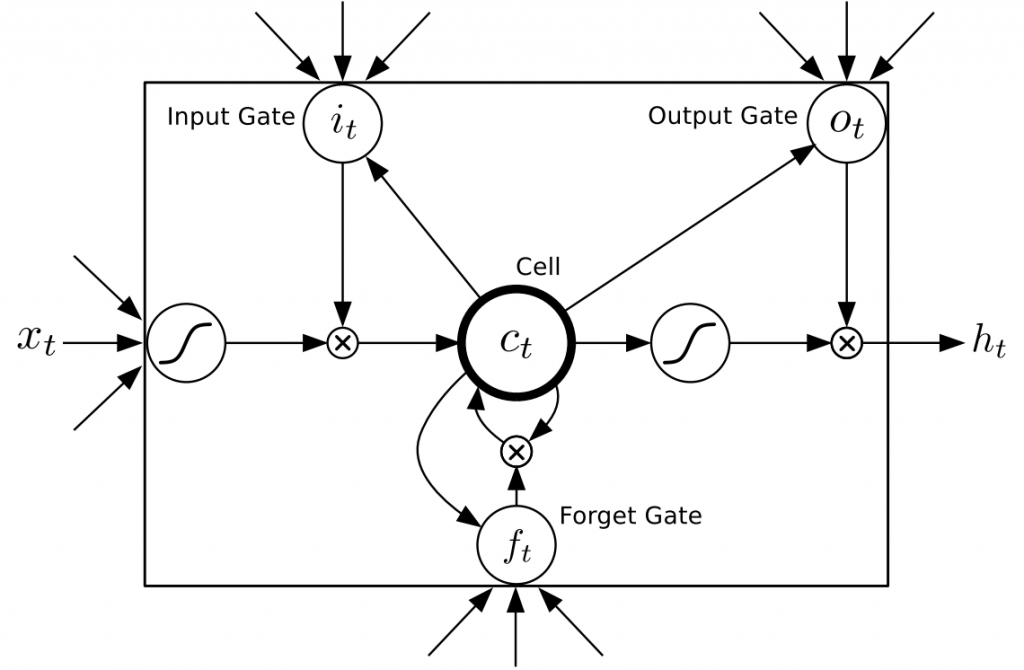
\includegraphics[width=0.45\textwidth]{lstm_cell.png}
            \caption{LSTM Cell Representation}
            \label{fig:lstm-cell}
        \end{figure}
        LSTM is a type of Recurrent Neural Network, specializing to work with long term dependencies. Typically, an LSTM network is composed of cells (depicted in figure \ref{fig:lstm-cell}) containing an input gate, output gate, forget gate, and at least one memory cell. The input gate controls what value can be entered into the memory cell, the output gate controls which of the values in the cell should be used, and forget gate controls which value in the cell should remain. By having such an architecture, a neural network utilizing the LSTM framework excels at understanding input information using what it has learned before, making it an ideal framework for audio analysis. The recent success in using Neural Networks for tasks such as speech recognition is due to this framework.
%%%%%%%%%%%%%%%%%%%%%%%%%%%%%%%%%%%%%%%%
%%%%% DATASET DESCRIPTION AND ANALYSIS
%%%%%%%%%%%%%%%%%%%%%%%%%%%%%%%%%%%%%%%%
\section{DATASET DESCRIPTION AND ANALYSIS}
The discussion in this section covers the datasets that were used for obtaining the training data, how the training data used in our research was selected from these datasets, and the preprocessing methods used before feeding the data into the neural network. 

%%%%%%%%%%%%%%%%%%%%%%%%%%%%%%%%%%%%%%%%
%%%%% DATASETS USED
%%%%%%%%%%%%%%%%%%%%%%%%%%%%%%%%%%%%%%%%
    \subsection{DATASETS USED}
        \begin{figure}[H]
            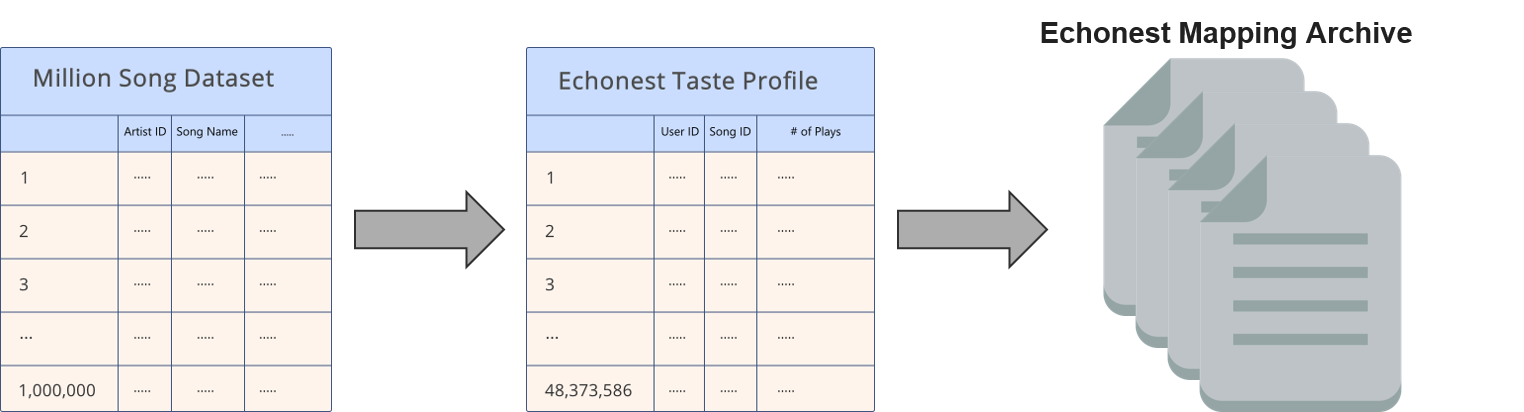
\includegraphics[width=0.45\textwidth]{dataset_mapping.png}
            \caption{Simple Graphic Displaying Datasets}
            \label{fig:datasets}
        \end{figure}

        \subsubsection{Million Song Dataset}
            The Million Song Dataset (depicted on the left in Figure \ref{fig:datasets}) is a dataset containing various fields of metadata for popular songs. \cite{msd_site} The data includes information such as the song title, artist name, album title, as well as more in depth information like the tempo of the song (BPM) and the estimated musical key that the song is played in. Many other researchers have used this dataset and it's subsets to perform music recommendation related research. \cite{Wang2014,Wang:2014:ICH:2647868.2654940,NIPS2013_5004} Unfortunately, all of the data provided by the subset is unusable for the purposes of the experiments performed here as no real-world user data is provided. However The EchoNest Taste Profile Subset provides this information and will be discussed next.
        \subsubsection{The EchoNest Taste Profile Subset}
        The EchoNest Taste Profile Subset (depicted int the center of Figure \ref{fig:datasets}) provides play count information using 384,546 songs of the Million Song Dataset for 1,019,318 prior EchoNest users. \cite{etp_site} There is a total of 48,373,586 records that contain the EchoNest song ID, the user ID of the user playing that song and the number of times that user played a song. This information is immensely useful for researchers that wish to perform a music recommendation analysis, or in our case, estimate how many times a user is likely to play a given song. 
        
        With the limited ability of real-world user data that is readily available via APIs due to permissions needed to access a user's information on popular music services, this archive is very valuable for research. For example, Spotify's API requires explicit permission for a user to simply read a user's recently played and top played tracks. \cite{spotify_permissions} Even then, these API queries are limited to 50 songs maximum, and are not guaranteed to not contain duplicates. \cite{spotify_recent,spotify_top} 
        \subsubsection{Echonest Mapping Archive}
        Due to the acquisition of The EchoNest by Spotify and it's subsequent shutdown, it is no longer possible to easily map the songs available in The EchoNest Taste Profile Subset or Million Song Dataset to other music services as this functionality was removed. However, a group of researchers created the The EchoNest Mapping Archive (depicted on the right in Figure \ref{fig:datasets}) that maps the songs includen in the Million Song Dataset to many other music services such such as Spotify, 7-Digital, MusiXMatch, and others in an archive of individual JSON files. \cite{map_site} Without this dataset, the only way to map between services would be by querying using Artist and Song names which is not guaranteed to provide accurate results. It is worth noting that the archive is not 100\% complete. In our experiments, we were able to obtain between 40\% and 60\% of the Spotify IDs for songs we obtained during data extraction.
        
%%%%%%%%%%%%%%%%%%%%%%%%%%%%%%%%%%%%%%%%
%%%%% TRAINING DATA EXTRACTION
%%%%%%%%%%%%%%%%%%%%%%%%%%%%%%%%%%%%%%%%
    \subsection{TRAINING DATA EXTRACTION}
    The final set of data that was used for training and evaluating our network models was obtained primarily from The EchoNest Taste Profile Subset and secondarily from The EchoNest Mapping Archive. The triplets from The EchoNest Taste Profile Subset were loaded into a MySQL database and results were obtained after various queries narrowing down the dataset to an acceptable level based on alloted computation time and storage space. These queries are explained in the below subsections. Once the final records were obtained, The EchoNest Mapping Archive JSONs were queried to obtain the corresponding Spotify IDs, added to a Spotify Playlist using the Spotify API and music data was obtained using a Spotify Premium Membership.
        \subsubsection{Limiting Maximum Number of Plays}
        After initially examining the dataset, it appeared that there were quite a few outliers due to some play counts. Some records showed over 1000 plays for a single user/song pair, so it was decided to trim outliers from the dataset by limiting the maximum number of plays per record to 200 plays. In total this trimmed the entire dataset from approximately 48 million records down to 48,370,466.
        \subsubsection{Obtaining the Top 5 Users}
        From the trimmed dataset, the top 5 users were selected based on the total aggregate number of plays. These were obtained using an SQL query to sum the number of plays, grouped by User ID. The decision to choose the top 5 users was done in order to be able to provide a comparison of network structures for multiple users and to see whether or not a model exists that performs universally acceptably. The decision to only perform network training on the data for 5 users was due again to limited training time and storage budgets.
        \subsubsection{Choosing Training Data}
        The final data set used for training the networks was obtained by querying the database for all songs listened to by at least two of the top 5 users. This resulted in a total of 341 songs, of which only 150 had corresponding Spotify IDs in The EchoNest Mapping Archive JSON files. These Spotify IDs were then added to a Spotify Playlist and the audio files were downloaded using a Spotify Premium Membership.
        
%%%%%%%%%%%%%%%%%%%%%%%%%%%%%%%%%%%%%%%%
%%%%% DATA PREPARATION
%%%%%%%%%%%%%%%%%%%%%%%%%%%%%%%%%%%%%%%%
    \subsection{DATA PREPARATION}
    This subsection describes how the user and audio data were treated during the training process and the preprocessing methods used before feeding in the data to the network.
        \subsubsection{User Play Information}
        Of the 341 final songs selected, a CSV file was generated for each user containing the records for that User ID with each record consisting of the User ID, Song EchoNest ID, and number of plays. In order to be able to compare the performance per user directly, the column of user plays was standardized for each user before being used as training data by the network. The function in Algorithm \ref{alg:load-userdata} was implemented for loading and preprocessing the user data. 
        \begin{algorithm}[h]
            \KwIn{Location of User Data, Location of Music Data}
            \KwOut{Tuples of (User ID, Song ID, Standardized Play Value)}
            \SetKwProg{function}{load\_and\_preprocess\_user\_data}{end}
            \function{
                $userData$ = read user record CSV file\\
                $musicAvailable$ = list songs in music directory\\
                \ForAll{song $s$ in $userData$}{
                 \If{ Song $s$ is not in $musicAvailable$}{
                      Remove $s$ from $userData$
                  }
                 }
                 Standardize number-of-plays column in userData\\
                 \Return userData
            }
        \caption{Load and Standardize User Data}
        \label{alg:load-userdata}
        \end{algorithm}

        \subsubsection{Audio Data}
        In order to make the network compatible with songs of varying length as well as make recommendations based on partial song information, the input to the network was limited to 5 second song clips. As will be explained in Section \ref{sec:nn-models}, the number of these 5 second vectors consumed by the network varied based on the network architecture, however each individual clip was no longer than 5 seconds. In order to process the audio files, two domain-specific Python libraries were employed: PyDub and LibROSA. \cite{librosa-site,pydub-site} In this case, PyDub was used to split the songs into their 5 second increments (depicted in figure \ref{fig:audio-split}) and LibROSA was used to convert the split MP3 files into NumPy arrays.
        \begin{figure}[H]
            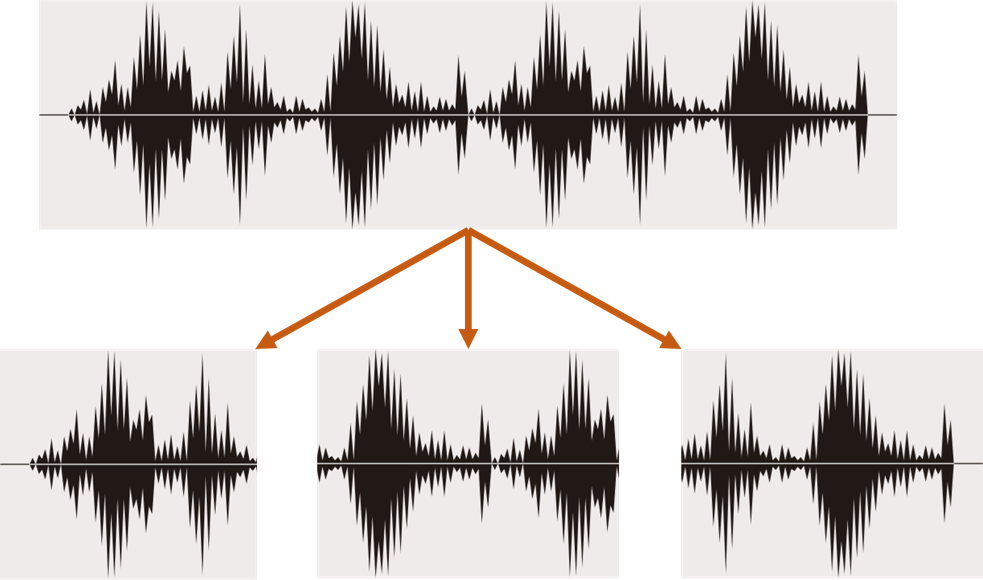
\includegraphics[width=0.45\textwidth]{song_split.png}
              \caption{Figure Depicting Audio Split}
              \label{fig:audio-split}
        \end{figure}

%%%%%%%%%%%%%%%%%%%%%%%%%%%%%%%%%%%%%%%%
%%%%% NEURAL NETWORK MODELS
%%%%%%%%%%%%%%%%%%%%%%%%%%%%%%%%%%%%%%%%
\section{NEURAL NETWORK MODELS} \label{sec:nn-models}

%%%%%%%%%%%%%%%%%%%%%%%%%%%%%%%%%%%%%%%%
%%%%% SOFTWARE AND HARDWARE USED
%%%%%%%%%%%%%%%%%%%%%%%%%%%%%%%%%%%%%%%%
    \subsection{Software and Hardware Used}
    For defining and training the models, Keras 2.1.4 was used with Tensorflow 1.7 on four AWS Elastic Cloud Compute (EC2) AMI instances. Keras was used in order to streamline the process of creating and defining the neural networks. The loaded music data was split into 90\% training and 10\% validation (the low ratio of validation to training data was due to having a small dataset) and each network was trained on 100 epochs with sample sets being shuffled in between each epoch.
    
    The choice between one or two LSTM layers as well as the input tensor of the network was defined at runtime using parameters passed to the Python script. The following subsections will explain in detail the concept of preparing the input data as well as the exact definitions of 'data vector', 'time steps', 'training samples', and 'input tensor' for the purposes of this paper.
    
%%%%%%%%%%%%%%%%%%%%%%%%%%%%%%%%%%%%%%%%
%%%%% LSTM INPUT STRUCTURE
%%%%%%%%%%%%%%%%%%%%%%%%%%%%%%%%%%%%%%%%
    \subsection{LSTM Input Structure}
     The following algorithm (\ref{alg:load-music}) walks through the pseudocode used to load the audio data into the accepted input tensor based on the parameters passed to the python script.
     
        \begin{algorithm}[h]
            \KwIn{Pre-processed user data, music data location, number of time steps}
            \KwOut{Tensor of dimensions: (training samples, time steps, data vector), Vector or matrix of target values}
            \SetKwProg{function}{load\_music}{end}
            \function{
                $targets$ = empty list\\
                $inputTensor$ = empty list\\
                \ForAll{songs $s$ in $userData$}{
                    $segmentList$ = sorted list of segments in song directory\\
                    $trainingSamplesForSong$ = floor($\frac{\text{length}(segmentList)}{timeSteps}$)\\
                    \For{$i$ in range(0, $trainingSamplesForSong$)}{
                        append $target$ to $targets$\\
                        $currTrainingSample$ = empty list\\
                        $currentClip$ = $i$ * $timeSteps$ \\
                        \For{$j$ in range($currentClip$, $currentClip + timeSteps$)}{
                            load and append column of segment data to $currTrainingSample$
                        }
                     append $currentTrainingSample$ to $inputTensor$ in 3rd dimension  
                    }
                 }
                 \Return $inputTensor$, $targets$
            }
        \caption{Load Music and Target Tensors}
        \label{alg:load-music}
        \end{algorithm}
     
        \subsubsection{Data Vector}
        The phrases 'data vector' or 'clip' refer to the NumPy array of a 5 second audio segment of the song. For example, a 60 second song would be broken up into twelve 5 second clips or data vectors. The reason for this explicit explanation is due to the Keras LSTM input shape definition which uses the phrase 'time steps' to refer to a different concept. In the case that a song was not evenly divisible into 5 second clips, the remainder of the final clip was expanded to 5 seconds by adding silence to the remainder of the clip.
        \subsubsection{Time Steps}
        When calling the Python script to begin training the neural network, the second parameter passed determines the number of time steps that will be used in the network. In this case the phrase 'time step' refers to the number of 5 second clips that are passed as a single training sample to the network. For example, a network with three time steps in the input shape will take in three 5 second clips as a single training sample. In the experiments run, the number of time steps was varied between 1 and 24 as the longest song available was only about 2 minutes long.
        \subsubsection{Training Samples}
        The number of training samples fed into the network was determined by both the number of songs and the length of each individual song. Due to this, each training sample for a single song would be treated as an individual song, except in the case that the song was only long enough to create a single training sample. As an example, if a song was 15 seconds long and the number of time steps was set to 1, then that song would be broken up into 3 training samples, as shown in figure \ref{fig:time-1}. As another example, if a particular song was 45 seconds long and the number of time steps was set to 3, then one would end up with 3 training samples for that song, each with three 5 second clips, as displayed by figure \ref{fig:time-3}, and this song's target would be added 3 times into the targets vector, with each training sample being treated individually.
            \begin{figure}
                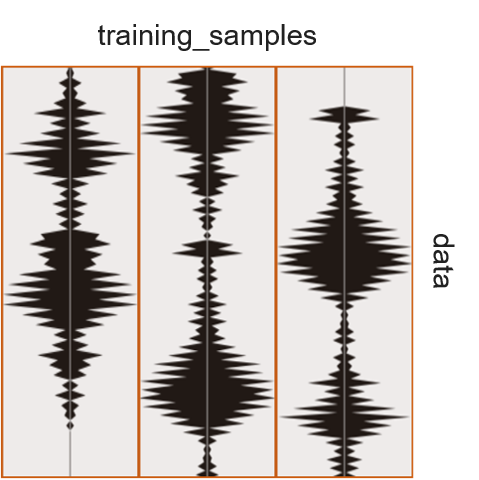
\includegraphics[width=0.45\textwidth]{1_time_step.png}
                \caption{Depiction of Input Using a Single Time Step}
                \label{fig:time-1}
            \end{figure}
            \begin{figure}
                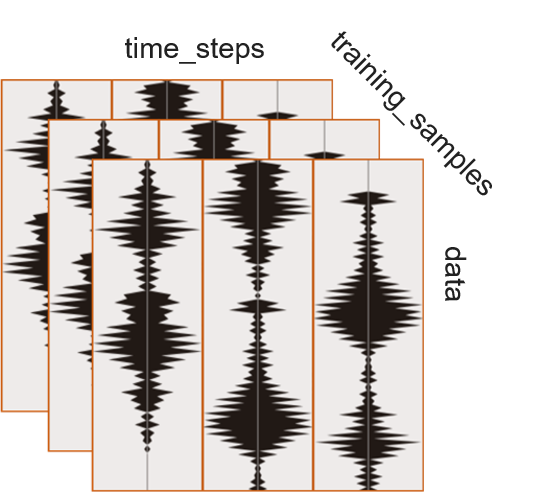
\includegraphics[width=0.45\textwidth]{3_time_steps.png}
                \caption{Depiction of Input Using 3 Time Steps}
                \label{fig:time-3}
            \end{figure}
            
%%%%%%%%%%%%%%%%%%%%%%%%%%%%%%%%%%%%%%%%
%%%%% MODELS USED
%%%%%%%%%%%%%%%%%%%%%%%%%%%%%%%%%%%%%%%%            
    \subsection{Models Used}
    For the experiments, as described at the beginning of the section, two different model shapes were used. First was a single LSTM layer with input shape defined as described previously, followed by a dense layer with a single output node depicted by figure \ref{fig:lstm-1}. The second network architecture used was simply adding another LSTM layer in between the first layer and dense layer as shown in figure \ref{fig:lstm-2}.
            \begin{figure}
                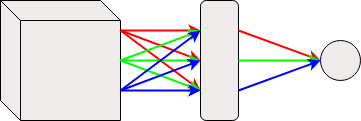
\includegraphics[width=0.45\textwidth]{lstm_single_layer.png}
                \caption{1-Layer LSTM Model}
                \label{fig:lstm-1}
            \end{figure}
            \begin{figure}
                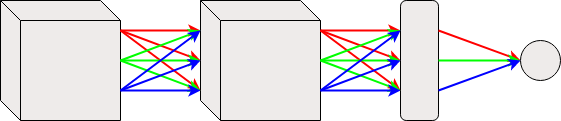
\includegraphics[width=0.45\textwidth]{lstm_2_layer.png}
                \caption{2-Layer LSTM Model}
                \label{fig:lstm-2}
            \end{figure}

%%%%%%%%%%%%%%%%%%%%%%%%%%%%%%%%%%%%%%%%
%%%%% RESULTS
%%%%%%%%%%%%%%%%%%%%%%%%%%%%%%%%%%%%%%%%
\section{RESULTS}
	In this section, we discuss the results for each model type: single layer and two layer LSTM, the model that performed best 'universally' across almost every user, the best performing model per user, and the best performing models for a single user (User 3). User 3 was chosen not because they had the best performance out of all users, as User 2 had that distinction, but rather User 3 has a balance of significant improvement and performance. An examination of poor performance is also included as to be transparent and address criticisms of our approach. 
    It is worth noting that for all of the following figures and discussions, the metric for the loss is the mean squared error (MSE) of the standardized play counts. In other words, an MSE of 1 means that the error by the network was $\pm1$ standard deviation. Over all experiments, user 1 had the worst performance, with no final MSE being under 1 standard deviation.
    
%%%%%%%%%%%%%%%%%%%%%%%%%%%%%%%%%%%%%%%%
%%%%% 1 LAYER
%%%%%%%%%%%%%%%%%%%%%%%%%%%%%%%%%%%%%%%%
	\subsection{Single Layer Model Results}
    Depicted in figure \ref{fig:results-1-layer} is the single layer LSTM model that had the best improvement for each user. These models are not necessarily the ones with the best performance overall. As can be seen, the number of time steps varied greatly, however in the majority of cases, the best improvements came from models with $\geq 10$ time steps. In this case, excluding User 1, the MSE for each model was $<1$ standard deviation.
        \begin{figure}
            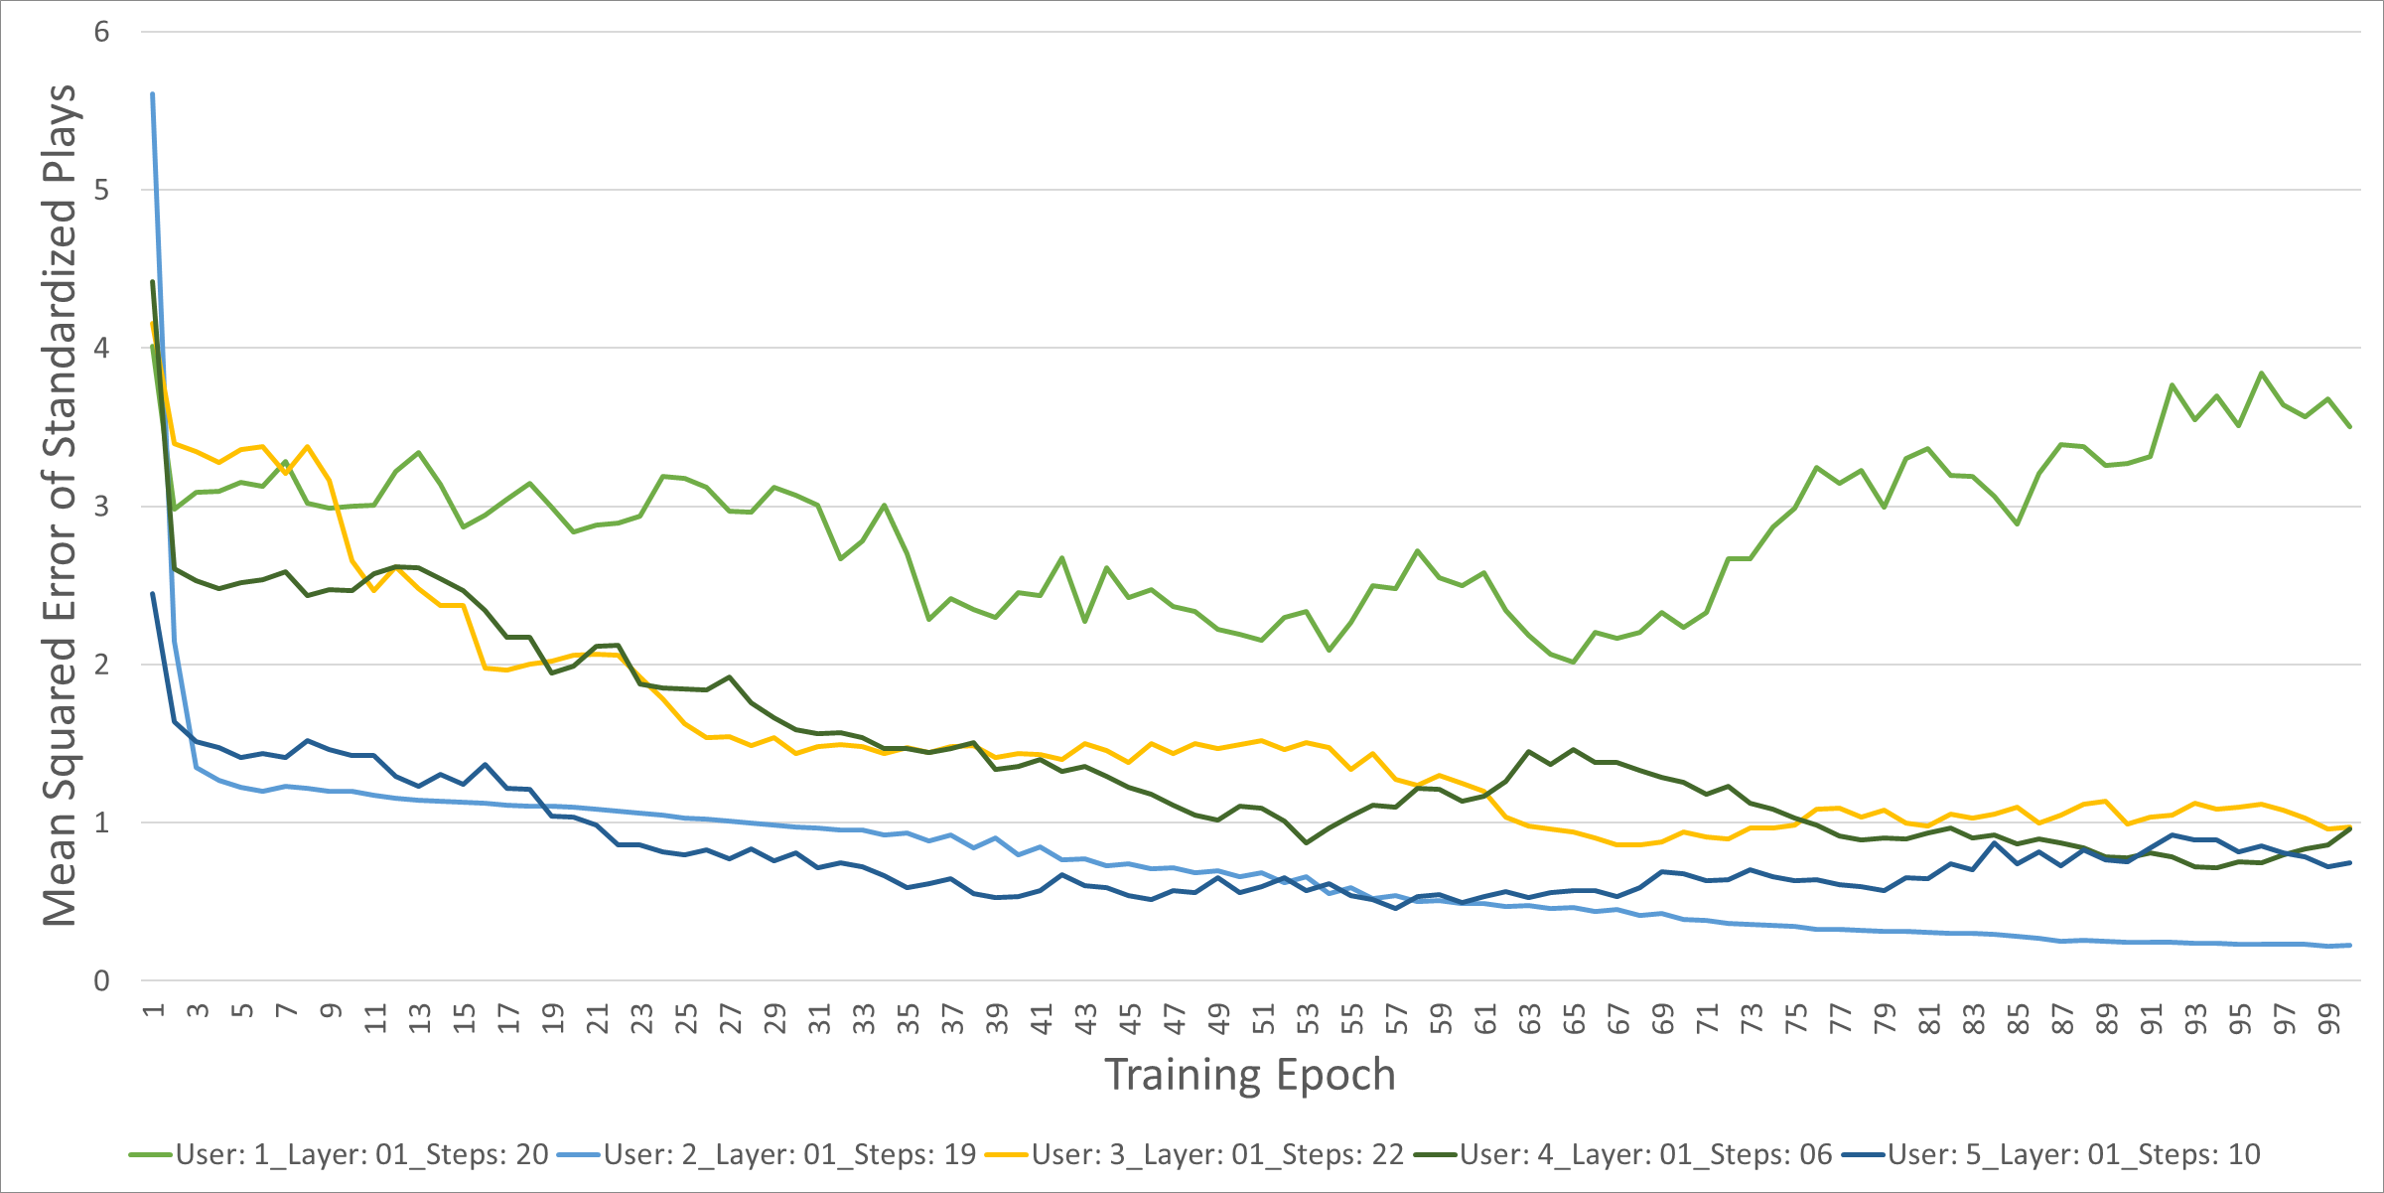
\includegraphics[width=0.45\textwidth]{result_best_1_layer.png}
            \caption{Best Performing Single LSTM Layer Model Per User}
            \label{fig:results-1-layer}
        \end{figure}
        
%%%%%%%%%%%%%%%%%%%%%%%%%%%%%%%%%%%%%%%%
%%%%% 2 LAYERS
%%%%%%%%%%%%%%%%%%%%%%%%%%%%%%%%%%%%%%%%
    \subsection{Two Layer Model Results}
    Similar to the prior subsection, figure \ref{fig:results-2-layer} displays the two layer models with the most improvement per user. As can be seen, in most cases the performance of the two layer LSTM models is significantly better than the single layer models. Excluding User 1, all of these models use $\geq 16$ time steps, further indicating that a longer time history improves the performance of the network.
        \begin{figure}
            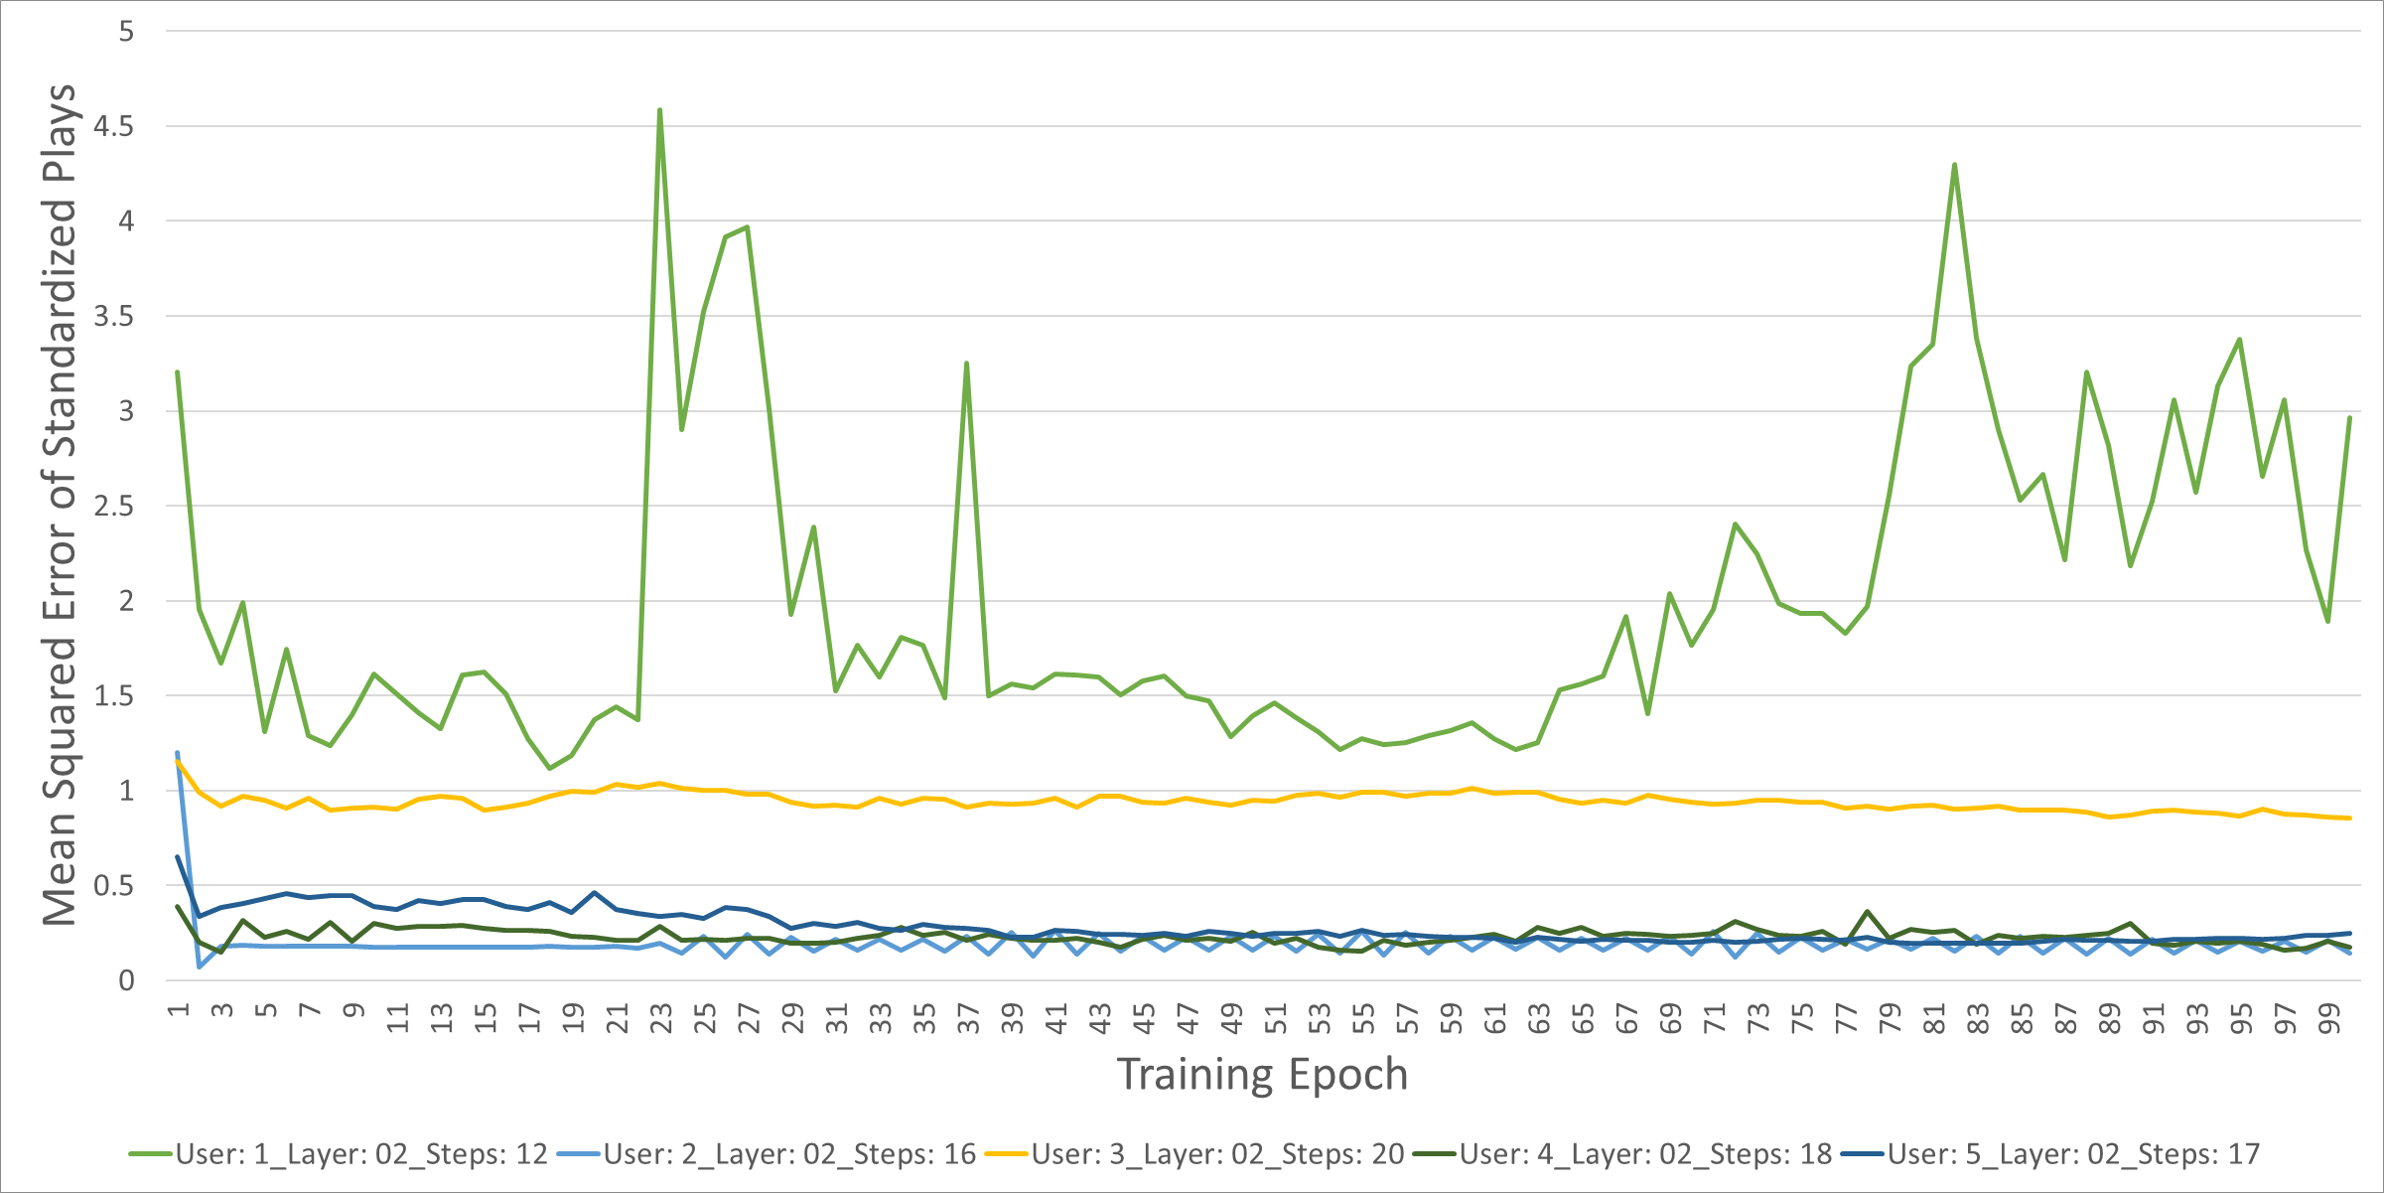
\includegraphics[width=0.45\textwidth]{result_best_2_layer.png}
            \caption{Best Performing Two LSTM Layer Model Per User}
            \label{fig:results-2-layer}
        \end{figure}
        
%%%%%%%%%%%%%%%%%%%%%%%%%%%%%%%%%%%%%%%%
%%%%% UNIVERSAL
%%%%%%%%%%%%%%%%%%%%%%%%%%%%%%%%%%%%%%%%  
    \subsection{Universal Model}
    While no model performed best for every single user, the combination of two LSTM layers and 18 time steps was the closest model to achieving that goal and the performance of this model is plotted in figure \ref{fig:results-overall}. In this case User 1's performance was divergent, however all other users had a final MSE of $<1$ and User 2-4 had a final MSE $<0.4$ standard deviations. Once again, this supports the assumption that a larger history for the LSTM to consider provides better performance.
        \begin{figure}
            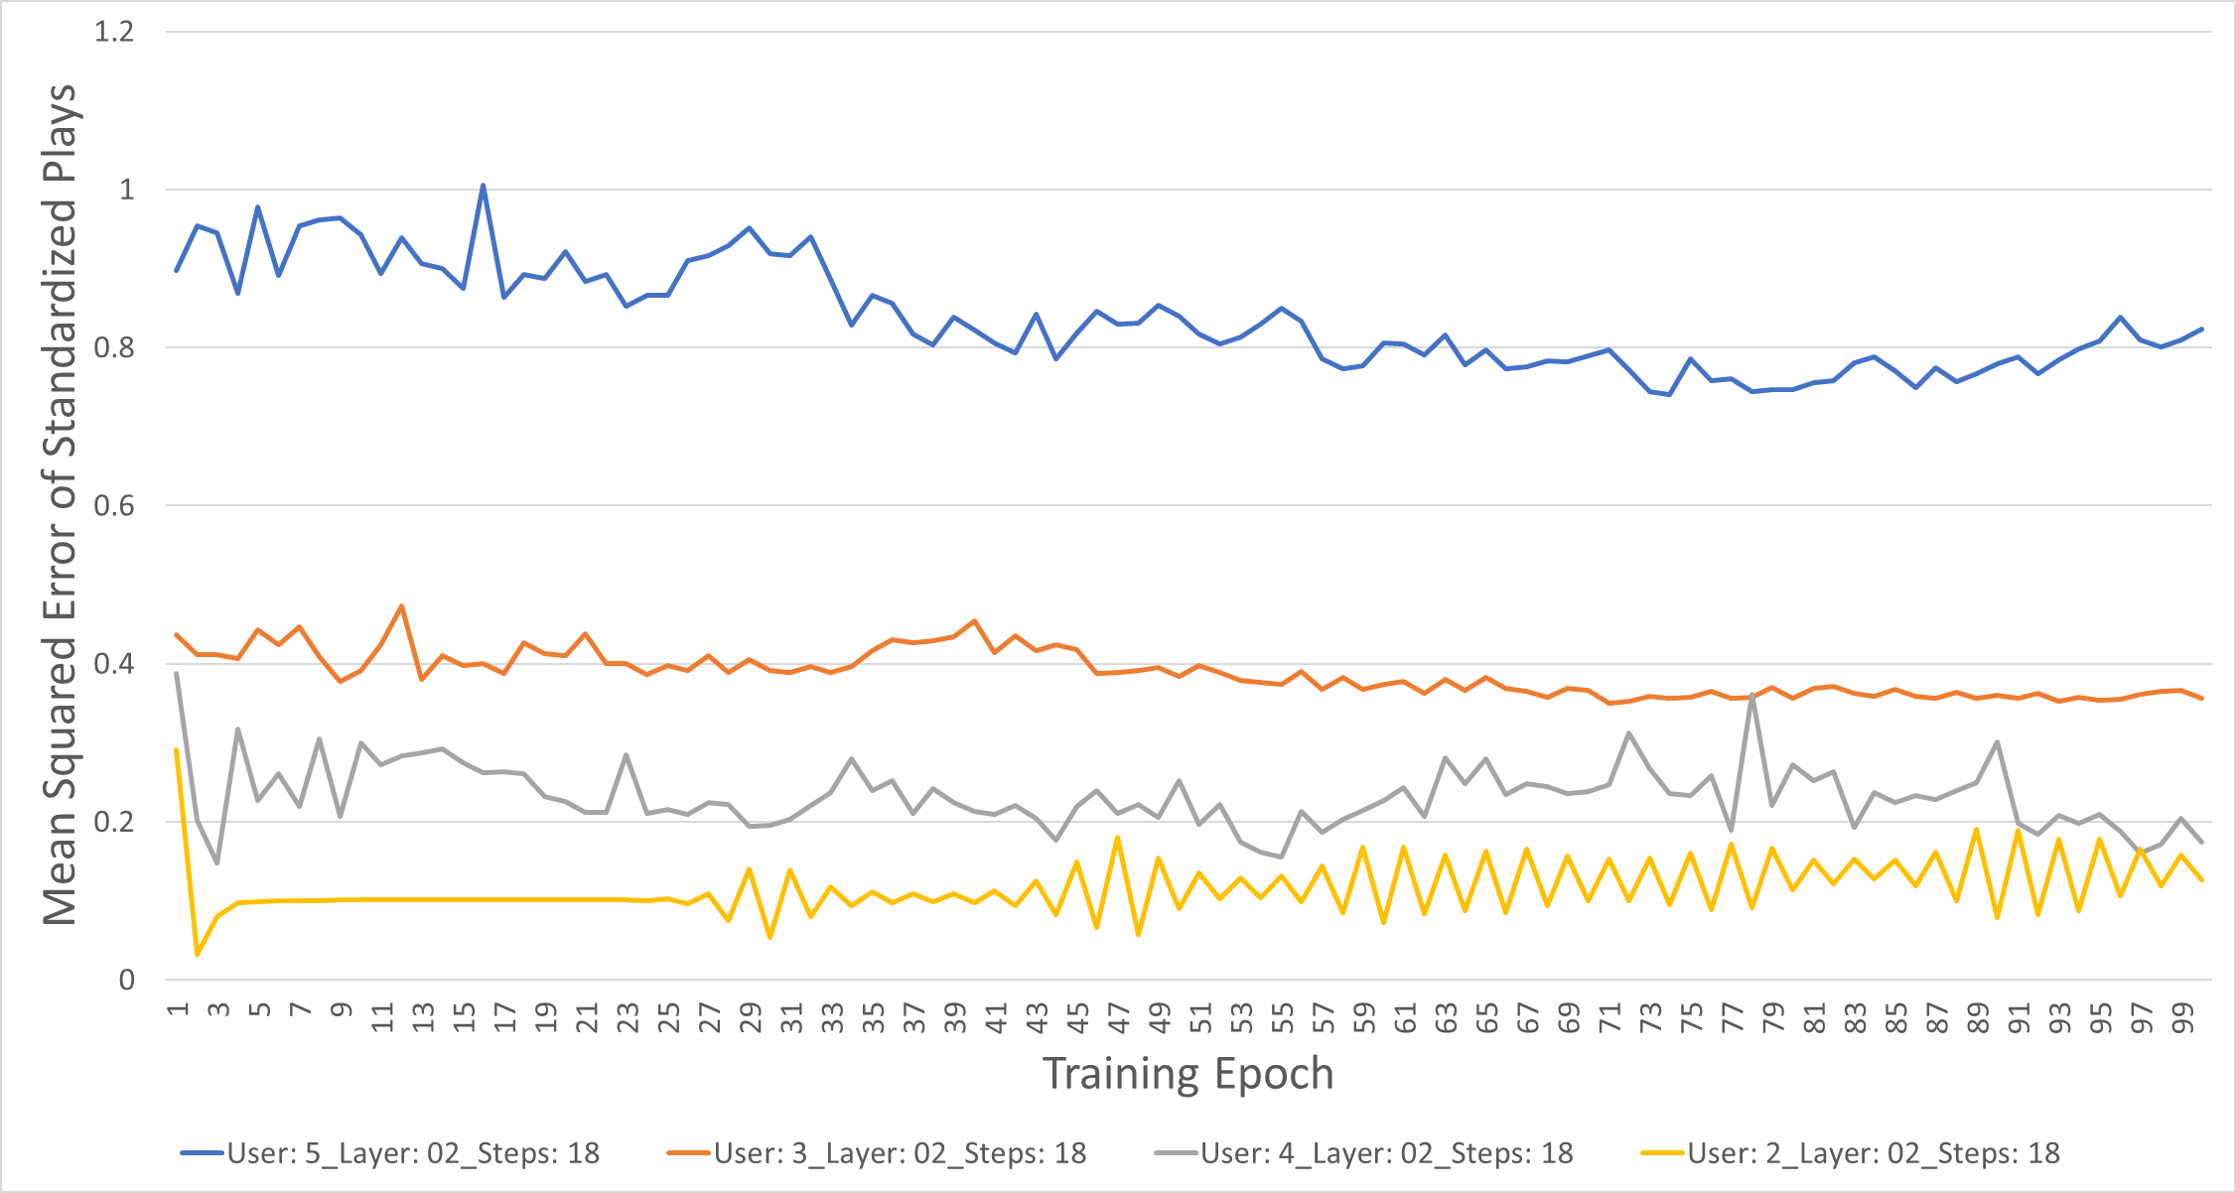
\includegraphics[width=0.45\textwidth]{result_best_overall.png}
            \caption{Best Universally Performing Model: 2 Layers 18 Time Steps}
            \label{fig:results-overall}
        \end{figure}
      
%%%%%%%%%%%%%%%%%%%%%%%%%%%%%%%%%%%%%%%%
%%%%% BEST PER USER
%%%%%%%%%%%%%%%%%%%%%%%%%%%%%%%%%%%%%%%%
    \subsection{Best Model Per User}
    Next we examine the best models in terms of performance per user and a sample of models for User 3 demonstrating excellent improvement and overall performance. Firstly, in figure \ref{fig:results-best-per-user}, for Users 2-5, the final performance was MSE $<0.4$, which is better than a random guess at the standardized number of plays for that user. User 5 had the best performance of all users, with the best performing model having a MSE $<0.06$.
        \begin{figure}
            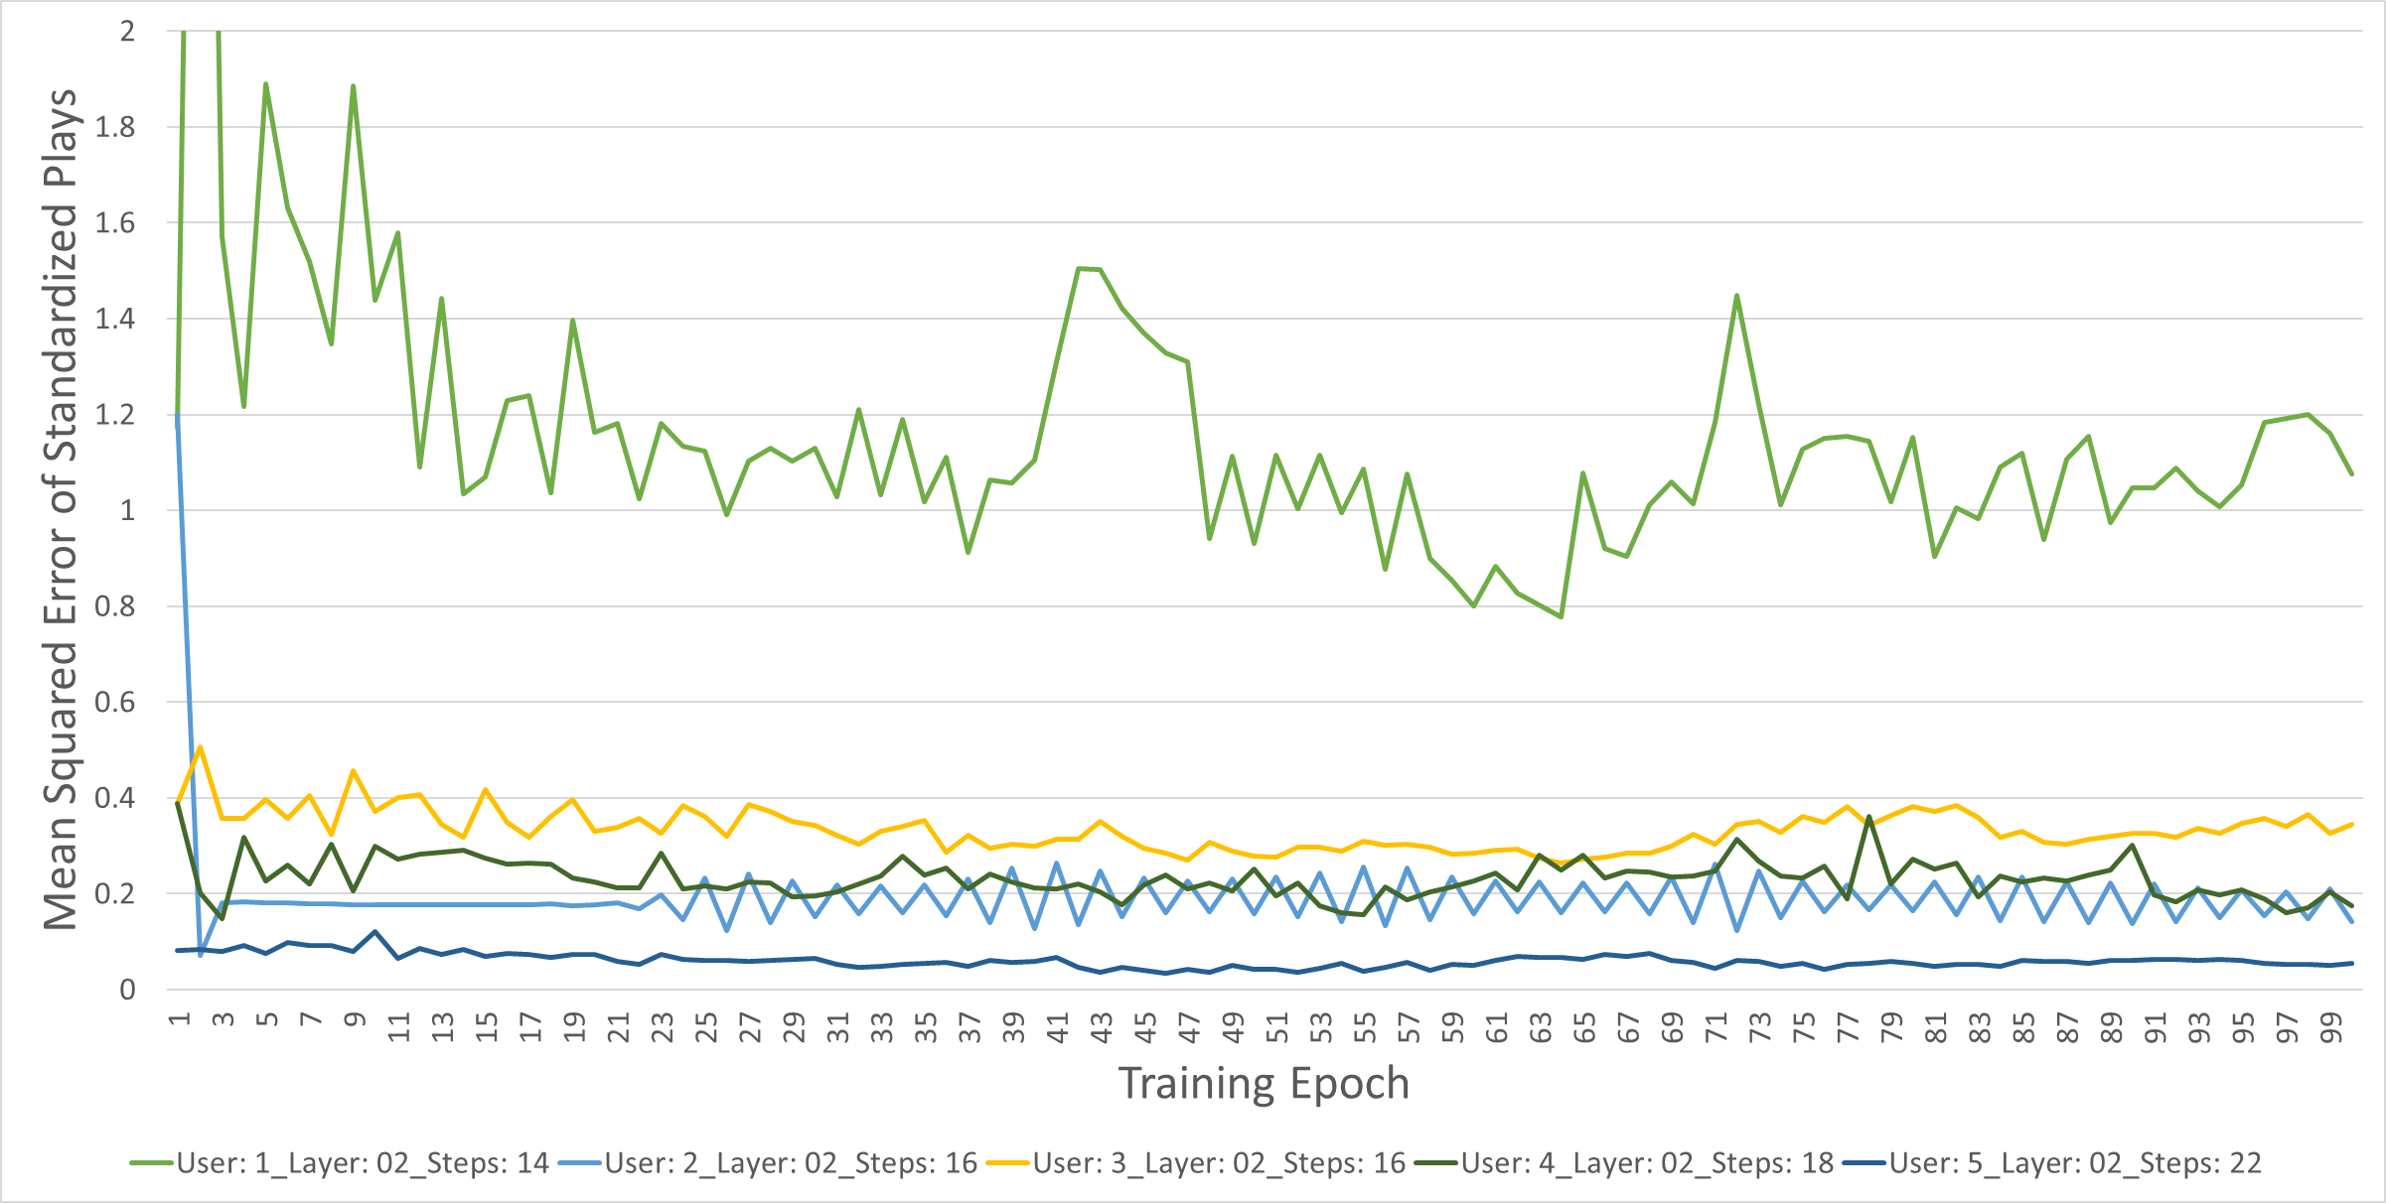
\includegraphics[width=0.45\textwidth]{result_best_per_user.png}
            \caption{Best Performing Model Per User}
            \label{fig:results-best-per-user}
        \end{figure}
        
    In figure \ref{fig:results-user-3}, multiple combinations of models are displayed over all 100 training epochs. In this case, the best performing models were under 0.5 MSE, however all models converged to an MSE of $<1$ standard deviation. The combination of 1 LSTM layer and 22 Time Steps is particularly impressive, converging to $<1$ MSE from $>4.15$ MSE at the first iteration.
        \begin{figure}
            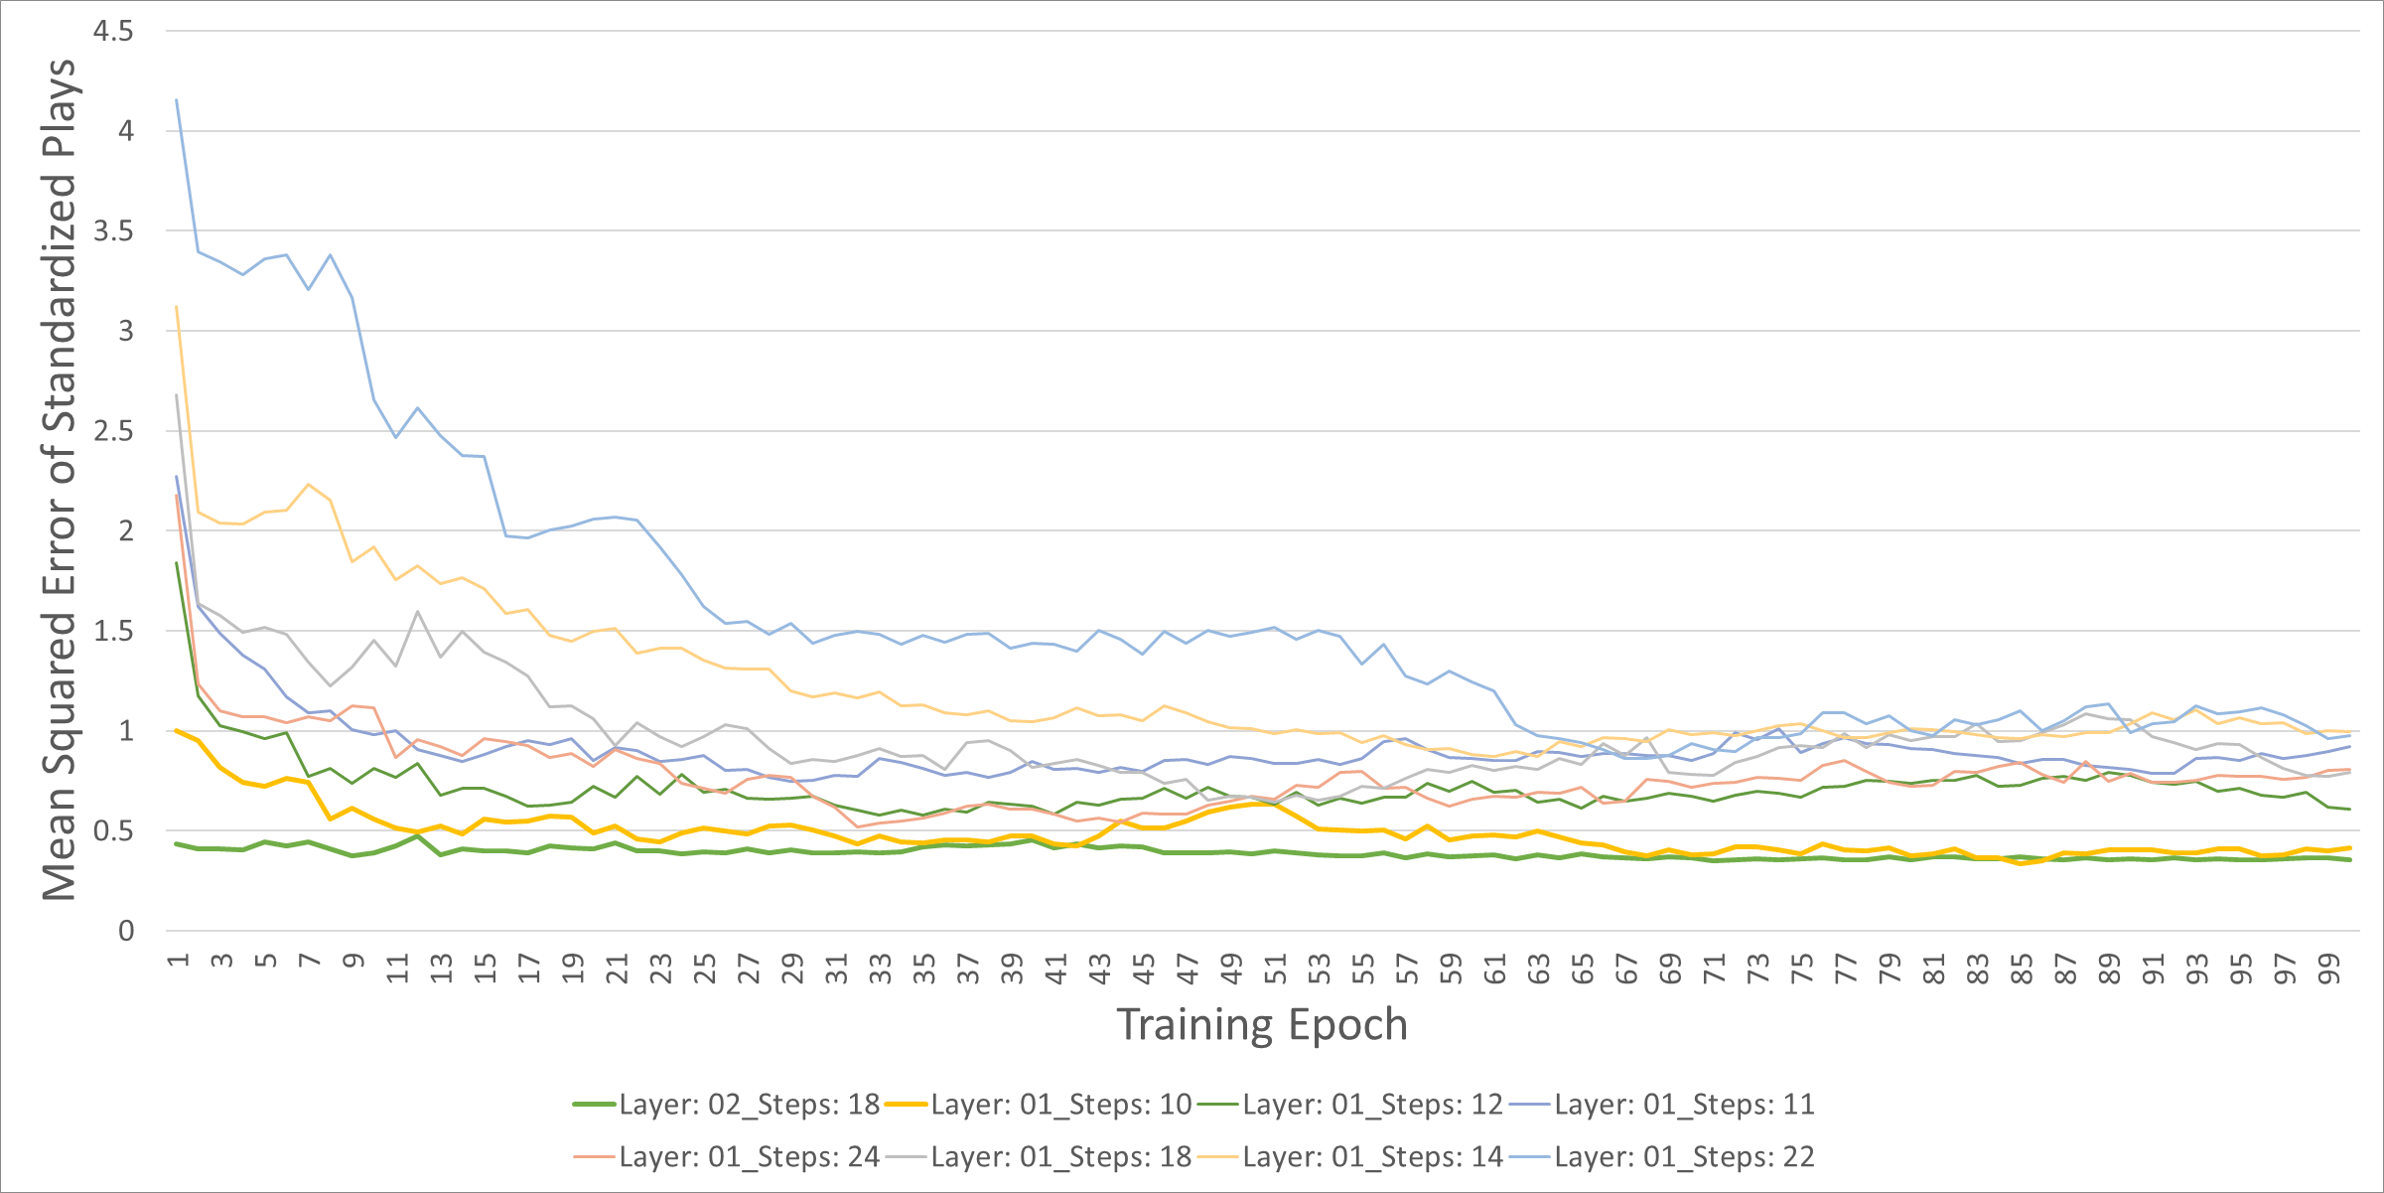
\includegraphics[width=0.45\textwidth]{result_user_3.png}
            \caption{Sample of Model Performance for User 3}
            \label{fig:results-user-3}
        \end{figure}
        
%%%%%%%%%%%%%%%%%%%%%%%%%%%%%%%%%%%%%%%%
%%%%% CRITICISMS
%%%%%%%%%%%%%%%%%%%%%%%%%%%%%%%%%%%%%%%%
    \subsection{Criticisms}
    For all users, there were some model combinations that had diverging loss, most commonly when the number of time steps was low. The researchers assume that this is due to the nature and purpose of LSTM networks, a longer time step (history) creates better performance. After all, the goal is to learn a pattern over time and remember that pattern to make predictions.  However, it is worth noting that this was not true 100\% of the time.  As one can see in figure \ref{fig:results-divergent}, these low time-step models provide poor performance and a divergent mean squared error. Some models even with larger time step values also performed poorly, most likely due to a bad random initialization.
        \begin{figure}
            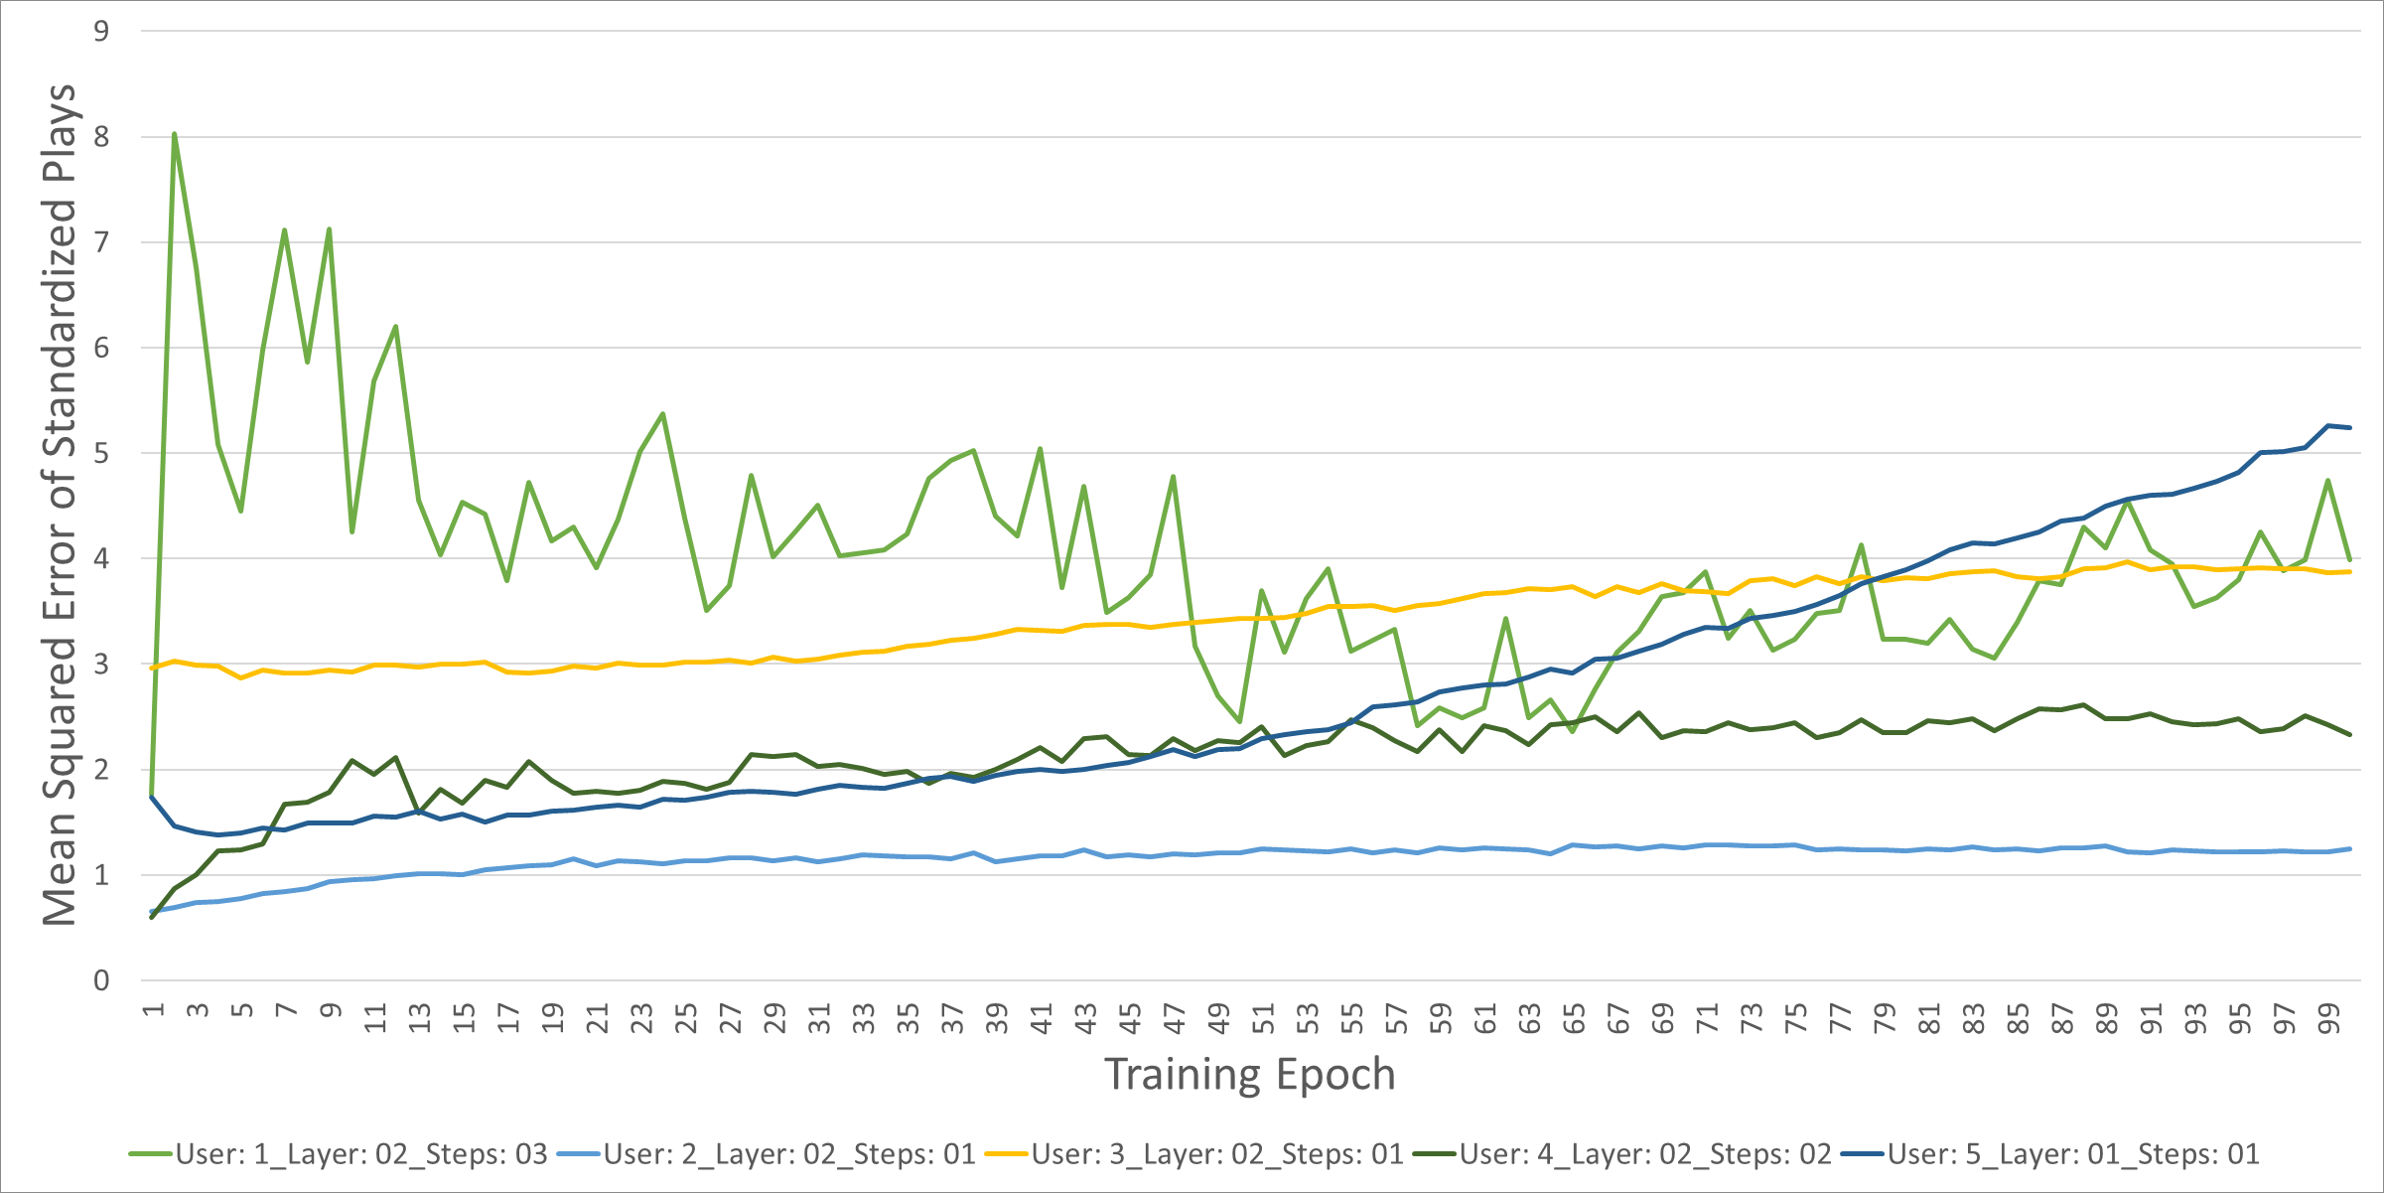
\includegraphics[width=0.45\textwidth]{result_diverging.png}
            \caption{Examples of Divergent Models Due to Too Few Time Steps}
            \label{fig:results-divergent}
        \end{figure}

%%%%%%%%%%%%%%%%%%%%%%%%%%%%%%%%%%%%%%%%
%%%%% CONCLUSION
%%%%%%%%%%%%%%%%%%%%%%%%%%%%%%%%%%%%%%%%
\section{CONCLUSION}
Most research in the field of music recommendation relies on binary classification or categorizing music into clusters. While there has been success in this area, many of these methods still rely heavily on metadata to accomplish their goal.\cite{Wang2014,Wang:2014:ICH:2647868.2654940} Although the success of our experiments was relatively minor considering the constraints that time and budget imposed on the amount of data that was able to be processed, the results were fairly promising and indicate that further research can be fruitful.

As stated, our goal was to find a method to assist current music recommendation systems while being metadata agnostic. Agnosticism of information such as the musician(s) responsible for writing a song creates potential for new artists to be recommended equally as well established ones, in essence creating a level playing field in the market and a lower barrier to entry. The content-based nature of the neural network creates an environment in which latent features may be extracted regardless of genre or artist and theoretically allow users to expand the repertoire of music that they enjoy. In addition, the focus on predicting the number of times a user will play a song potentially allows the distribution service, record label, and music artists to increase revenue.
%%%%%%%%%%%%%%%%%%%%%%%%%%%%%%%%%%%%%%%%
%%%%% FUTURE WORK
%%%%%%%%%%%%%%%%%%%%%%%%%%%%%%%%%%%%%%%%
\section{FUTURE WORK}
The following suggestions for improvement of the developed system could prove to be fruitful paths to take.
\begin{itemize}
	\item Attempting to use a deeper or varied network:
		\begin{itemize}
			\item Adding more LSTM Layers
            \item Adding more LSTM layers with the number of hidden neurons cascading
            \item Using more fully connected layers with a slower reduction to one output neuron
            \item Allowing dropout internally in the LSTM layers or in the dense layers
            \item Using an autoencoder to preprocess audio data before feeding into the LSTM network.
		\end{itemize}
	\item Increasing the amount of data for training the networks
    \item Using different loss functions than MSE
    \item Using different activation functions other than sigmoid in the neural network
    \item Use only a single time step with multiple networks and averaging the result of all networks
\end{itemize}

%%%%%%%%%%%%%%%%%%%%%%%%%%%%%%%%%%%%%%%%%%%%%%%%%%%%%%%%%%%%%%%%%%%%%%%%%%%%%%%%%%%%%%%%%%%%%%%%%%%%%%%%%%%%%%%%%%%%%%%%%%%
%%%%% APPENDIX
%%%%%%%%%%%%%%%%%%%%%%%%%%%%%%%%%%%%%%%%%%%%%%%%%%%%%%%%%%%%%%%%%%%%%%%%%%%%%%%%%%%%%%%%%%%%%%%%%%%%%%%%%%%%%%%%%%%%%%%%%%%
\section*{Appendix A}
All source code used for the project can be obtained from \href{https://github.com/ttakasawa/Music_Play_Count_Estimator}{GitHub - ttakasawa: Music Play Count Estimator}

%%%%%%%%%%%%%%%%%%%%%%%%%%%%%%%%%%%%%%%%%%%%%%%%%%%%%%%%%%%%%%%%%%%%%%%%%%%%%%%%%%%%%%%%%%%%%%%%%%%%%%%%%%%%%%%%%%%%%%%%%%%
%%%%% BIBLIOGRAPHY
%%%%%%%%%%%%%%%%%%%%%%%%%%%%%%%%%%%%%%%%%%%%%%%%%%%%%%%%%%%%%%%%%%%%%%%%%%%%%%%%%%%%%%%%%%%%%%%%%%%%%%%%%%%%%%%%%%%%%%%%%%%
\nocite{*}
\bibliographystyle{ACM-Reference-Format}
\bibliography{bibliography}


\end{document}
